\documentclass{article}
\usepackage{amsmath}
\usepackage{amsfonts}
\usepackage{amsthm}
\usepackage{empheq}
\usepackage{tikz}
\usepackage{enumitem}

\swapnumbers
\theoremstyle{definition}
\newtheorem{definicion}{Definición}[section]

\newcommand{\tagcirculo}[1]{%
  \begin{tikzpicture}[baseline=(node.base)]
    \node[circle, draw, inner sep=2pt, minimum size=0.2cm, thick] (node) {\small #1};
  \end{tikzpicture}%
}

\begin{document}

    \section{El operador diferencial en superficies}

    \begin{definicion}
      Sea $S \xrightarrow{f} R$ una función diferenciable entre superficies. 
      Para cada $\phi \in S$, el operador diferencial de $f$ en $\phi$ es la función $d f_\phi$, 
      que toma a cada vector $v = G'(t_0)$ tangente de una curva $G(t) \subseteq S$ que 
      pasa por $\phi = G(t_0)$, y lo manda en $\omega = \tau'(t_0)$ donde 
      $\tau(t) = f(G(t))$.
 
      \begin{center}
        \begin{equation*}
          \begin{aligned}
            d\, f_\phi: T_\phi(S) &\to T_{f(\phi)}(R) \\
              v = G'(t_0) &\to \omega = \tau'(t_0);\quad\quad \tau(l) = f(G(l))
          \end{aligned}
        \end{equation*}
      \end{center}
    \end{definicion}

  \vspace{1em}
    \subsection*{1.2 Escritura local:}
    \vspace{0.5em}

    \begin{center}
      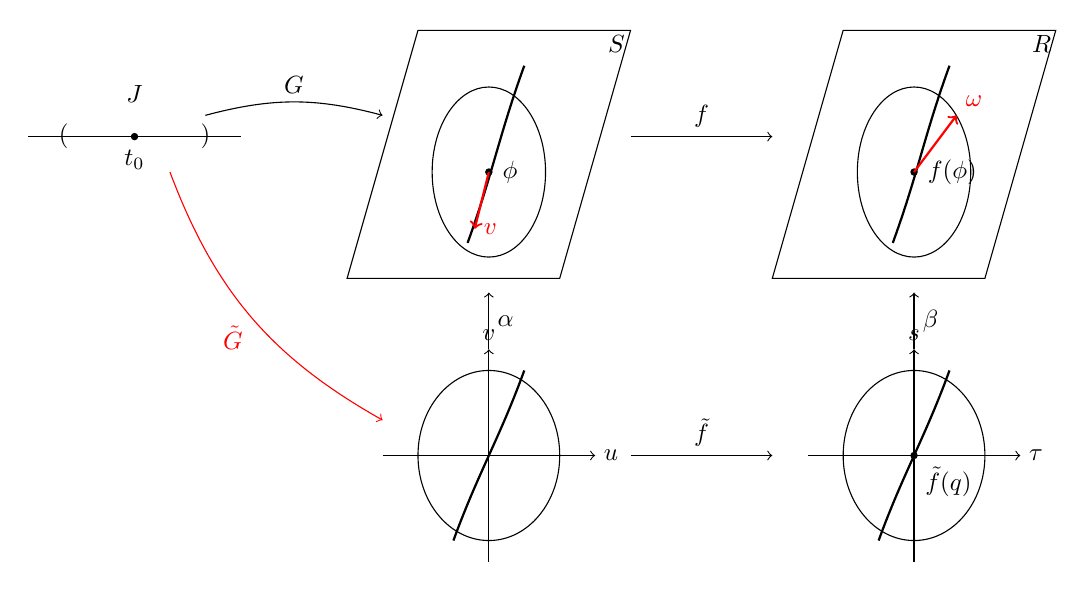
\begin{tikzpicture}[scale=0.9, every node/.style={scale=0.9}]

        \begin{scope}[shift={(0,4)}]

          \draw (-2,-1.5) -- (1,-1.5) -- (2,2) -- (-1,2) -- cycle;
          \node at (1.8, 1.8) {$S$};

          \draw (0,0) ellipse (0.8 and 1.2);

          \draw[thick] (-0.3,-1) to[out=70, in=250] (0.5,1.5);

          \fill (0,0) circle (1.5pt) node[right=2pt] {$\phi$};

          \draw[->, thick, red] (0,0) -- (-0.2,-0.8) node[right] {$v$};
        \end{scope}

        \begin{scope}[shift={(6,4)}]

          \draw (-2,-1.5) -- (1,-1.5) -- (2,2) -- (-1,2) -- cycle;
          \node at (1.8, 1.8) {$R$};

          \draw (0,0) ellipse (0.8 and 1.2);

          \draw[thick] (-0.3,-1) to[out=70, in=250] (0.5,1.5);

          \fill (0,0) circle (1.5pt) node[right=2pt] {$f(\phi)$};

          \draw[->, thick, red] (0,0) -- (0.6,0.8) node[above right] {$\omega$};
        \end{scope}


        \begin{scope}[shift={(-5,4.5)}]
          \draw (-1.5,0) -- (1.5,0);
          \node at (-1,0) {$($}; 
          \node at (1,0) {$)$};
          \fill (0,0) circle (1.5pt) node[below=2pt] {$t_0$};
          \node at (0,0.6) {$J$};
        \end{scope}


        \begin{scope}[shift={(0,0)}]

          \draw[->] (-1.5,0) -- (1.5,0) node[right] {$u$};
          \draw[->] (0,-1.5) -- (0,1.5) node[above] {$v$};

          \draw (0,0) ellipse (1 and 1.2);

          \draw[thick] (-0.5,-1.2) to[out=70, in=250] (0.5,1.2);
        \end{scope}

        \begin{scope}[shift={(6,0)}]

          \draw[->] (-1.5,0) -- (1.5,0) node[right] {$\tau$};
          \draw[->] (0,-1.5) -- (0,1.5) node[above] {$s$};

          \draw (0,0) ellipse (1 and 1.2);

          \draw[thick] (-0.5,-1.2) to[out=70, in=250] (0.5,1.2);
          \fill (0,0) circle (1.5pt) node[below right=1pt] {$\tilde{f}(q)$};
        \end{scope}

        \draw[->] (-4, 4.8) to[bend left=15] node[above] {$G$} (-1.5, 4.8);

        \draw[->, red] (-4.5, 4) to[bend right=20] node[below left] {$\tilde{G}$} (-1.5, 0.5);

        \draw[->] (2, 4.5) -- (4, 4.5) node[midway, above] {$f$};

        \draw[->] (2, 0) -- (4, 0) node[midway, above] {$\tilde{f}$};

        \draw[->] (0, 1.5) -- (0, 2.3) node[midway, right] {$\alpha$};

        \draw[->] (6, 1.5) -- (6, 2.3) node[midway, right] {$\beta$};

      \end{tikzpicture}
    \end{center}


    Tomemos $\epsilon > 0$ suficientemente pequeño, tal que en $(t_0 - \epsilon, t_0 + \epsilon)$ están
    definidas todas las siguientes funciones:
    \begin{equation*}
      \begin{aligned}
        \tilde{G}(l) &= \alpha^{-1} (G(l)) = (u(l), v(l)) \in U\quad\quad\quad &(U, \alpha) = \text{ corta en } \phi \\
        \tilde{f}(u, v) &= \beta^{-1} (f(\alpha(u, v))) = (\tau(u, v), S(u, v)) \in V \quad\quad\quad &(V, \beta) = \text{ "}\quad\text{"} f(\phi)
      \end{aligned}
    \end{equation*}

    Entonces,


    \begin{empheq}{align*}
        \tilde{\tau}(l) &= \beta^{-1}(\tau(l)) = \text{escritura local de } \tau(t) = f(G(l)) \\
        &= \beta^{-1}\, f\, G(l) = \beta^{-1}\, f\, (\alpha \tilde{G})(l) \\[0.5em] 
        \Aboxed{\tilde{\tau}(l) &= \tilde{f}(\tilde{G}(l)) = \bigl( \tau(u(l), v(l)), S(u(l), v(l)) \bigr)} 
        \stepcounter{equation}
        \tag{\tagcirculo{i}}
    \end{empheq}

    donde las funciones $\tau(u, v),\quad S(u, v), \quad u(l), \quad v(l)$ son todas diferenciables. En consecuencia; por la regla 
    de la cadena:

    \[
      \tilde{\tau}'(t_0) = \left[\tilde{f}(\tilde{G}(t_0))  \right] \cdot \left[\tilde{G}(t_0) \right] = 
      \left[
        \begin{aligned}
          &\tau_u (u_0, v_0) \quad &\tau_v (u_0, v_0) \\
          &S_u (u_0, v_0) \quad &S_v (u_0, v_0)
        \end{aligned}
      \right]
      \left(
        \begin{aligned}
          u'(t_0) \\
          v'(t_0)
        \end{aligned}
      \right)
      \stepcounter{equation}
      \tag{\tagcirculo{ii}}
    \]
  \section{Propiedades del operador diferencial:}

  \begin{itemize}[label=(\alph*)]
    \item \underline{$d\, f_\phi$ está bien definida}: Por las igualdades $\tag{\tagcirculo{iv}}$ y $\tag{\tagcirculo{v}}$, $d\, f_\phi(v)$
      solo depende de $\phi \in S$, la función $f$ y el vector $v \in T_p (S)$; \underline{no} \underline{de} \underline{la} \underline{curva} G(l). En 
          otras palabras, si $\eta(l)$ es otra curva tal que $\eta'(t_0) = v$ en $\eta(l) = \phi$, entonces 
          $d\, f_\phi (v) = \left.\frac{d}{d\,l}(f(\eta(l)))\right|_{l = t_0} = \left. \frac{d}{d\, l} (f(G(l))) \right|_{l = t_0}$
          da lo mismo.

    \item \underline{$d\, f_\phi$ es lineal:} (en $T_p(S)$) Por la estructura local,
          $d\, f_\phi: T_p(S) \to T_{f(\phi)}(R)$ satisface $d\, f_\phi (v) = A \cdot v$, donde 
          $A = \left[\tilde{f}_\phi\right](q)$ es la matriz Jacobiana de cualquier 
          escritura local $\tilde{f} = \beta^{-1} f \alpha$ de $f$ en $q = \alpha^{-1}(\phi)$. Entonces

          \begin{equation*}
            \begin{aligned}
              d\, f_\phi(c \cdot v + \omega) &= A(c \cdot v + \omega) = c(Av) + A\omega \\
              &= c d\, f_\phi(v) + d\, f_\phi(\omega)
            \end{aligned}
          \end{equation*}

    \item \underline{$d\, f_\phi$} \underline{no} \underline{depende de las cartas y escritura local}: Por 
          la manera en la que es definido en (1), no se emplea una carta local.
  \end{itemize}
\end{document}
